\texttt{Consegna}\\
Si richiede di realizzare una demo di animazione digitale 2D interattiva simile al materiale fornito.\\
Punti fondamentali del progetto:
\begin{itemize}
    \item l’impegno artistico e l’impatto visivo della scena
    \item la presenza e qualitá delle animazioni basate su simulazioni fisiche (es. uso leggi di cinematica/
dinamica)
    \item la presenza di elementi di gameplay con condizioni di vittoria/sconfitta per il giocatore
    \item l’utilizzo dei particellari nella scena
\end{itemize}
\texttt{Svolgimento}\\
Creazione di Arkanoid.\\
La demo creata consiste in un livello di Arkanoid, il cui scopo è colpire tutti i mattoncini con una palla. L'implementazione, in quanto doveva essere un breve gioco, consiste di un solo livello. \\
Analizzando ora tutti i punti fondamentali richiesti nel progetto:
\begin{itemize}
    \item Le animazioni che sono state utilizzate all'interno del gioco sono tre: il movimento della pallina quando rimbalza su una superficie, il movimento del giocatore, e la scomparsa di un blocco quando esso viene colpito.\\
    \begin{itemize}
        \item Per rendere la pallina controllabile, quando viene colpita dal giocatore, il nuovo angolo che avrà la pallina varia in base alla posizione di dove ha colpito il giocatore. È stata utilizzata la formula della interpolazione lineare per trovare il nuovo angolo. Per capire come è stata utilizzata la LERP per risolvere questo problema, è sufficiente consultare la funzione \textit{playerBallAngle}
        \item Il giocatore non ha accelerazione, ma si muove con velocità costante, altrimenti sarebbe incontrollabile e sarebbe impossibile colpire la pallina nel punto voluto
        \item I blocchi una volta colpiti, non scompaiono veramente, ma il loro colore diventa uguale a quello dello sfondo e non vengono più considerati gli impatti con quel blocco
    \end{itemize}
    \item Sinceramente, non trovo le particelle molto belle visivamente, ma data la richiesta, sono state emesse all'impatto della pallina con il giocatore.
    \item Ci sono due possibilità per il giocatore: vincere o perdere. In ogni caso, lo schermo finale sarà il medesimo, ma la prima possibilità la si ottiene colpendo tutti i blocchi, la seconda facendo cadere la pallina. Per conoscere il proprio punteggio è stato inserito lo score dei blocchi distrutti attualmente.\\
           {\centering
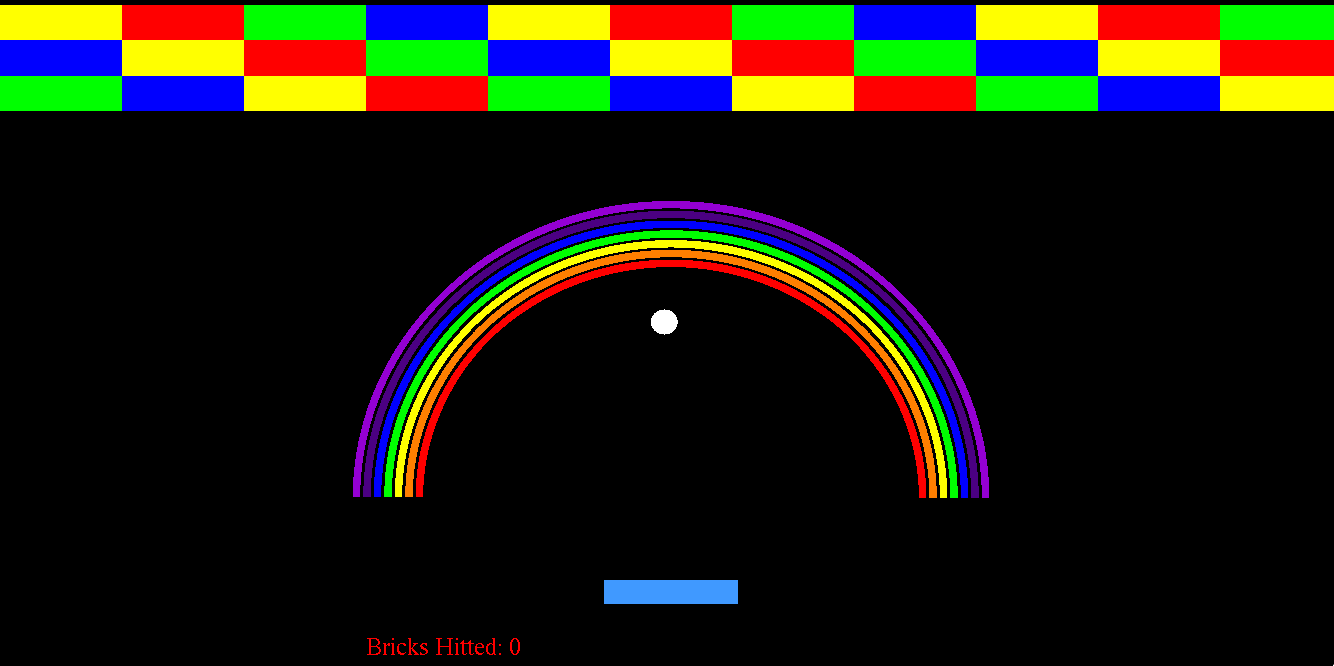
\includegraphics[width=0.6\textwidth]{arkanoin.png}} 
\end{itemize}